\chapter{Functional Mock-up Interface TLM Plugin}
Functional Mock-up Interface (FMI) is a tool-independent standard for connecting simulation tools \cite{blochwitz2009}. 
One tool can export a model as a Functional Mockup Unit (FMU), a ZIP package with the file extension FMU. 
This file is in turn loaded by the master simulation tool, which can connect and simulate the model.
An FMU file contains a model description XML file called \texttt{modelDescription.xml}, binaries for different platforms and other optional content.
It is important that the FMU contains a binary file for the platform where the master simulation tool is executed.

There are two versions of the FMI standard: FMI for Co-Simulation and FMI for Model Exchange.
The main difference is that FMUs for Co-Simulation contain their own built-in solvers, and only exchange data at predefined communication points.
FMUs for Model Exchange require a solver in the master simulation tool.

The TLM framework is able to simulate aggregated systems of connected sub-models using asynchronous TLM communication. 
Input, output and bidirectional interfaces are supported.
Bidirectional interfaces can be either 1D or 3D.
It is also possible to specifiy physical domains such as mechanical, rotational or hydraulic.
Including FMUs in the TLM framework requires a wrapper.
\texttt{FMIWrapper} is a generic wrapper for connecting functional mockup units (FMUs) to the TLM framework.
It uses the FMI Library from Modelon \cite{modelon2015} to load an FMU, and the TLMPlugin for socket communication with the framework, see figure \ref{fig:overview}.

\begin{figure}[ht]
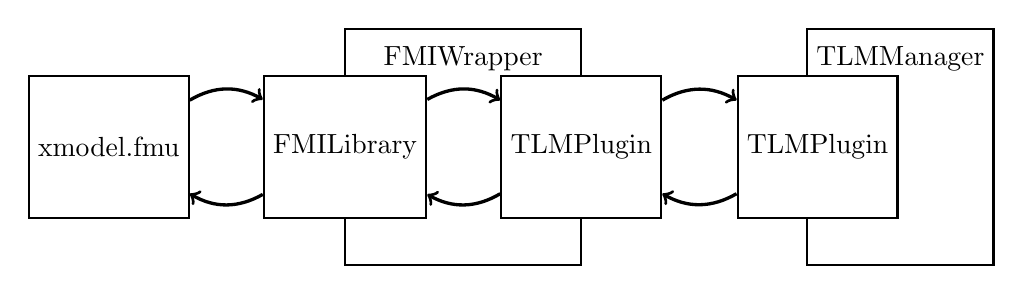
\begin{tikzpicture}
\def\dx{0.0495*\textwidth}

\node[rectangle,draw,thick, 
      minimum width=5*\dx, 
      minimum height=5*\dx, 
      text depth=5*\dx-20pt] () {FMIWrapper};

\node[rectangle, draw, thick, 
      minimum width=3*\dx, 
      minimum height=3*\dx, 
      xshift=2.5*\dx,
      fill=white] (tp1) {TLMPlugin};
      
\node[rectangle, draw, thick, 
      minimum width=3*\dx, 
      minimum height=3*\dx, 
      xshift=-2.5*\dx,
      fill=white] (fl) {FMILibrary};
      
\node[rectangle, draw, thick, 
      minimum width=3*\dx, 
      minimum height=3*\dx, 
      xshift=-7.5*\dx] (fmu) {xmodel.fmu};

\node[rectangle, draw, thick, 
      minimum width=3.5*\dx, 
      minimum height=5*\dx, 
      text depth=5*\dx-20pt,
      xshift=9.25*\dx,
      fill=white] () {TLMManager};

\node[rectangle, draw, thick, 
      minimum width=3*\dx, 
      minimum height=3*\dx, 
      xshift=7.5*\dx,
      fill=white] (tp2) {TLMPlugin};

\draw[thick,->,very thick] (fmu) edge[bend left] (fl);
\draw[thick,<-,very thick] (fmu) edge[bend right] (fl);
\draw[thick,->,very thick] (fl) edge[bend left] (tp1);
\draw[thick,<-,very thick] (fl) edge[bend right] (tp1);
\draw[thick,->,very thick] (tp1) edge[bend left] (tp2);
\draw[thick,<-,very thick] (tp1) edge[bend right] (tp2);
\end{tikzpicture}
\caption{FMIWrapper uses FMILibrary to import FMUs, and TLMPlugin for socket communication.}
\label{fig:overview}
\end{figure}

Both FMI for co-simulation and FMI for model exchange are supported. 
Model exchange requires a solver in the wrapper executable.
For this reason, the CVODE and IDA solvers from the Sundials package are included.
